\chapter{Rezultati}

S obzirom da CDH računalo nije dostupno u trenutku pisanja ovog rada,
komunikacija PDH računala s CDH računalom emulira se kroz komunikaciju s osobnim računalom
putem sučelja USART.
Na osobnom računalu potrebno je koristiti emulator terminala koji može koristiti UART komunikaciju. U tu svrhu odabran je program CoolTerm, 
koji može primati i slati podatke preko UART sučelja i može spremati  
primljene podatke, što je potrebno kako bi se na računalu mogla učitati slika s kamere. 
Brzina prijenosa putem UART sučelja postavljena je na 115200 bit/s.
Za obradu naredbi primljenih s osobnog računala korištena 
je programska potpora razvijena u okviru prethodnog rada \cite{diplomski_goran_petrak}.

Kada se sustav uključi prvo se ispisuje rezultat inicijalizacije sustava. Ako je inicijalizacija uspješna, ispisuje se poruka \verb|startup_ok|. Nakon toga nudi se izbor ponovne inicijalizacije datotečnog sustava, te se nudi izbor datoteke za slanje. Ako korisnik želi, može odmah nakon slanja datoteke odabranu datoteku izbrisati, a može i izbrisati datoteke bez prethodnog slanja. Korisnik može odabrati da se slanje datoteka preskoči. Sustav zatim traži od korisnika da koristi uobičajene, odnosne prethodne, postavke kamere ili da sam podesi postavke kamere ili da se korištenje kamere preskoči. Ako korisnik odabere da želi podesiti postavke kamere, sustav mu nudi da podesi vrijeme ekspozicije (\verb|nr_lines| za cjelobrojni dio i \verb|nr_lines_frac| za frakcionalni dio trajanja vremena ekspozicije), pojačanje pojačala (\verb|gain|) i format spremanja slike. Kada korisnik konfigurira postavke sustava i odabere željene funkcionalnosti,
sustav ponudi korisniku pokretanje operacija PDH sustava. Kada sustav završi s izvršavanjem operacija ispisuje se rezultat operacija i status sustava, te sustav krene ispočetka i ponovno ponudi korisniku reinicijalizaciju datotečnog sustava. Primjer komunikacije između računala i PDH sustava dan je u isječku koda \ref{lst:default_comms}.

\begin{minipage}{\linewidth}
\begin{lstlisting}[basicstyle=\tiny\ttfamily, caption=Komunikacija između računala i PDH sustava, label={lst:default_comms}]
sustav: startup_ok
sustav: Type 'reinit' to reinitialize the filesystem, 'n' not to
korisnik: n
sustav: Press 'y' to select file for transmission, 'n' to skip
korisnik: n
sustav: Any [other] file you would like to delete?['y'/'n']
korisnik: n
sustav: Press 'y' to set camera params, 'd' to use default/previous, 'n' to skip
korisnik: y
sustav: Set exposure nr_lines (uint16_t).
korisnik: 2000
sustav: Set exposure nr_lines frac (uint8_t).
korisnik: 10
sustav: Set gain (uint8_t), see acam.h.
korisnik: 9
sustav: Select format: 'r' for raw, 'j' for jpeg,
korisnik: j
sustav: Enter file name [0-1023] to store image measurments.
korisnik: 0
sustav: Press 's' to start PDH operations
korisni: s
sustav: Device camera status ok
sustav: Type 'reinit' to reinitialize the filesystem, 'n' not to
korisnik: n
sustav: Press 'y' to select file for transmission, 'n' to skip
korisnik: y
sustav: Enter file name [0-1023] of file to be transmitted via x-band.
korisnik: 0
sustav: Press 'y' to delete file after transmission, 'n' to keep it
korisnik: y
sustav: Any [other] file you would like to delete?['y'/'n']
korisnik: n
sustav: Press 'y' to set camera params, 'd' to use default/previous, 'n' to skip
korisnik: n
sustav: Press 's' to start PDH operations
korisnik: s
sustav: ÿØÿ
...
slanje slike
...
ÿÙ Device xband status ok
sustav: Type 'reinit' to reinitialize the filesystem, 'n' not to
\end{lstlisting}
\end{minipage}

Ovisno o svjetlini okoline gdje se nalazi kamera preporučuje se vrijednost cjelobrojnog dijela vremena ekspozicije 2000 za relativno svjetlo područje i 5000 za relativno mračno područje. Za frakcionalni dio vremena ekspozicije preporučuje se mala vrijednost, na primjer 10. Isto tako, male vrijednosti se preporučuju za pojačanje pojačala. Primjer slika koje su uslikane s navedenim parametrima u \textit{jpeg} formatu prikazane su na slikama \ref{fig:dark} i \ref{fig:light}.
\begin{figure}[H]
	\centering
	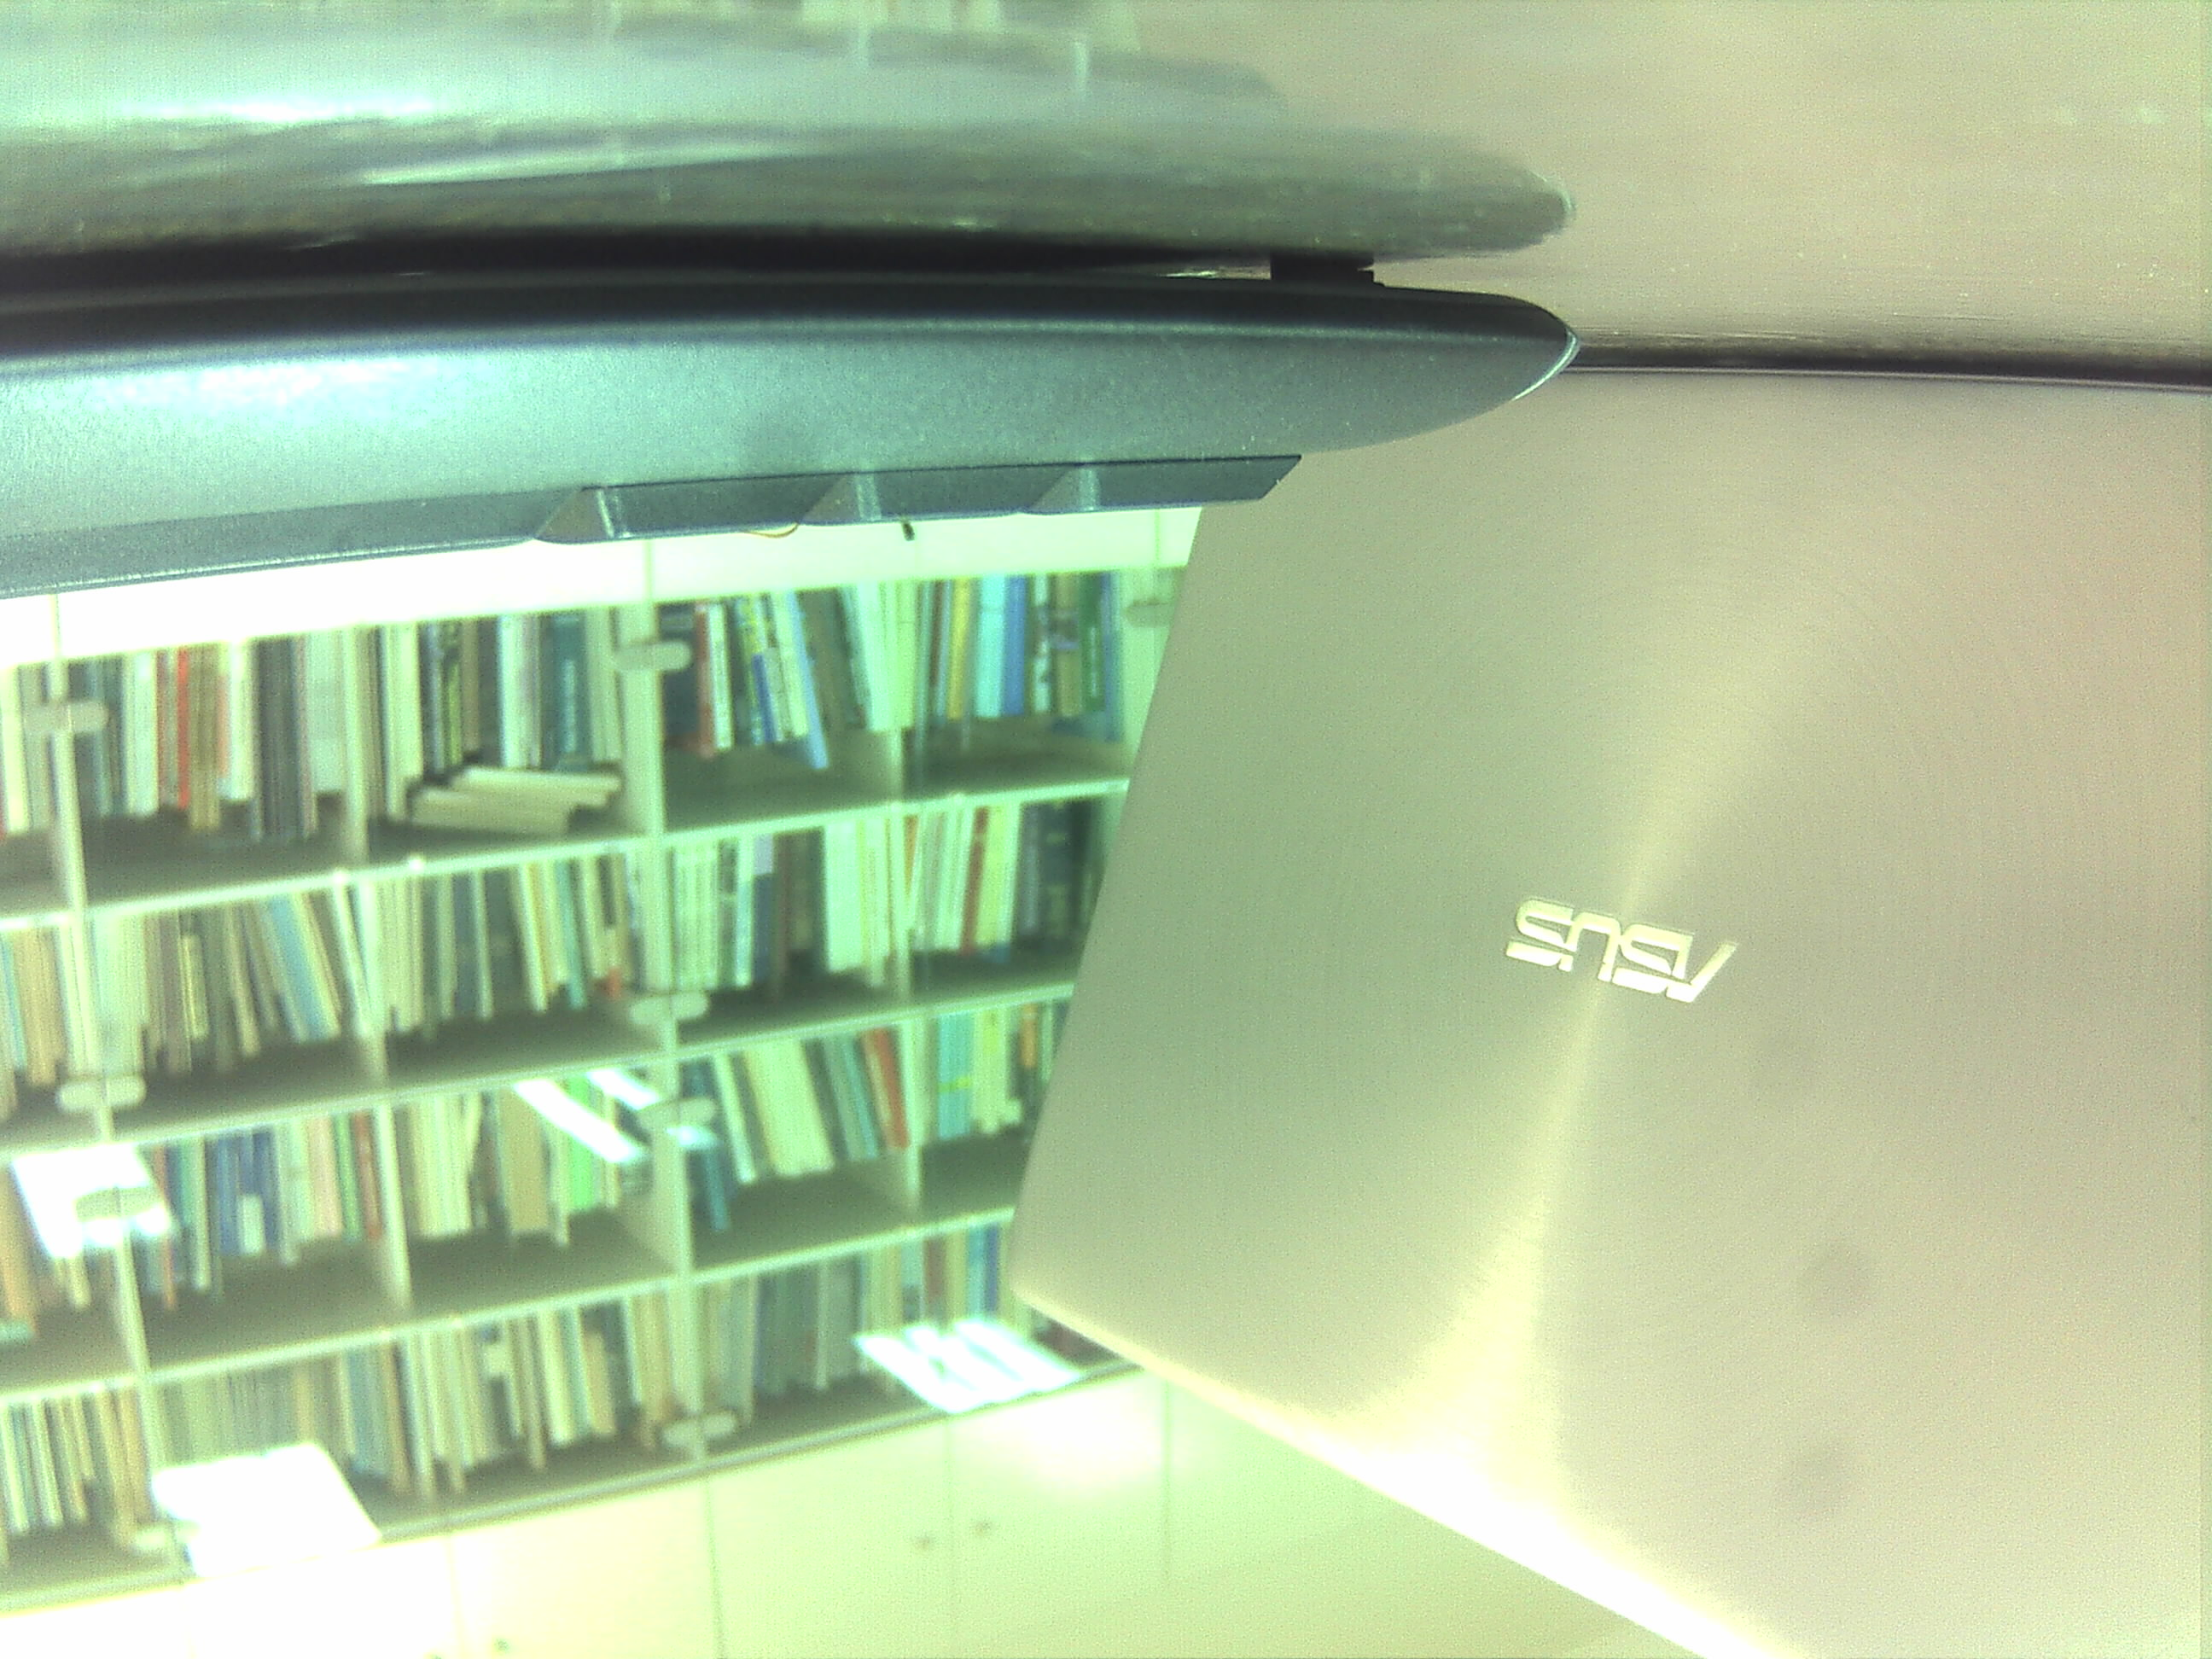
\includegraphics[height=5 cm, angle=180]{light.jpeg}
	\caption{Slika dobivena u relativno svjetlim uvjetima}
	\label{fig:light}
\end{figure}
\begin{figure}[H]
	\centering
	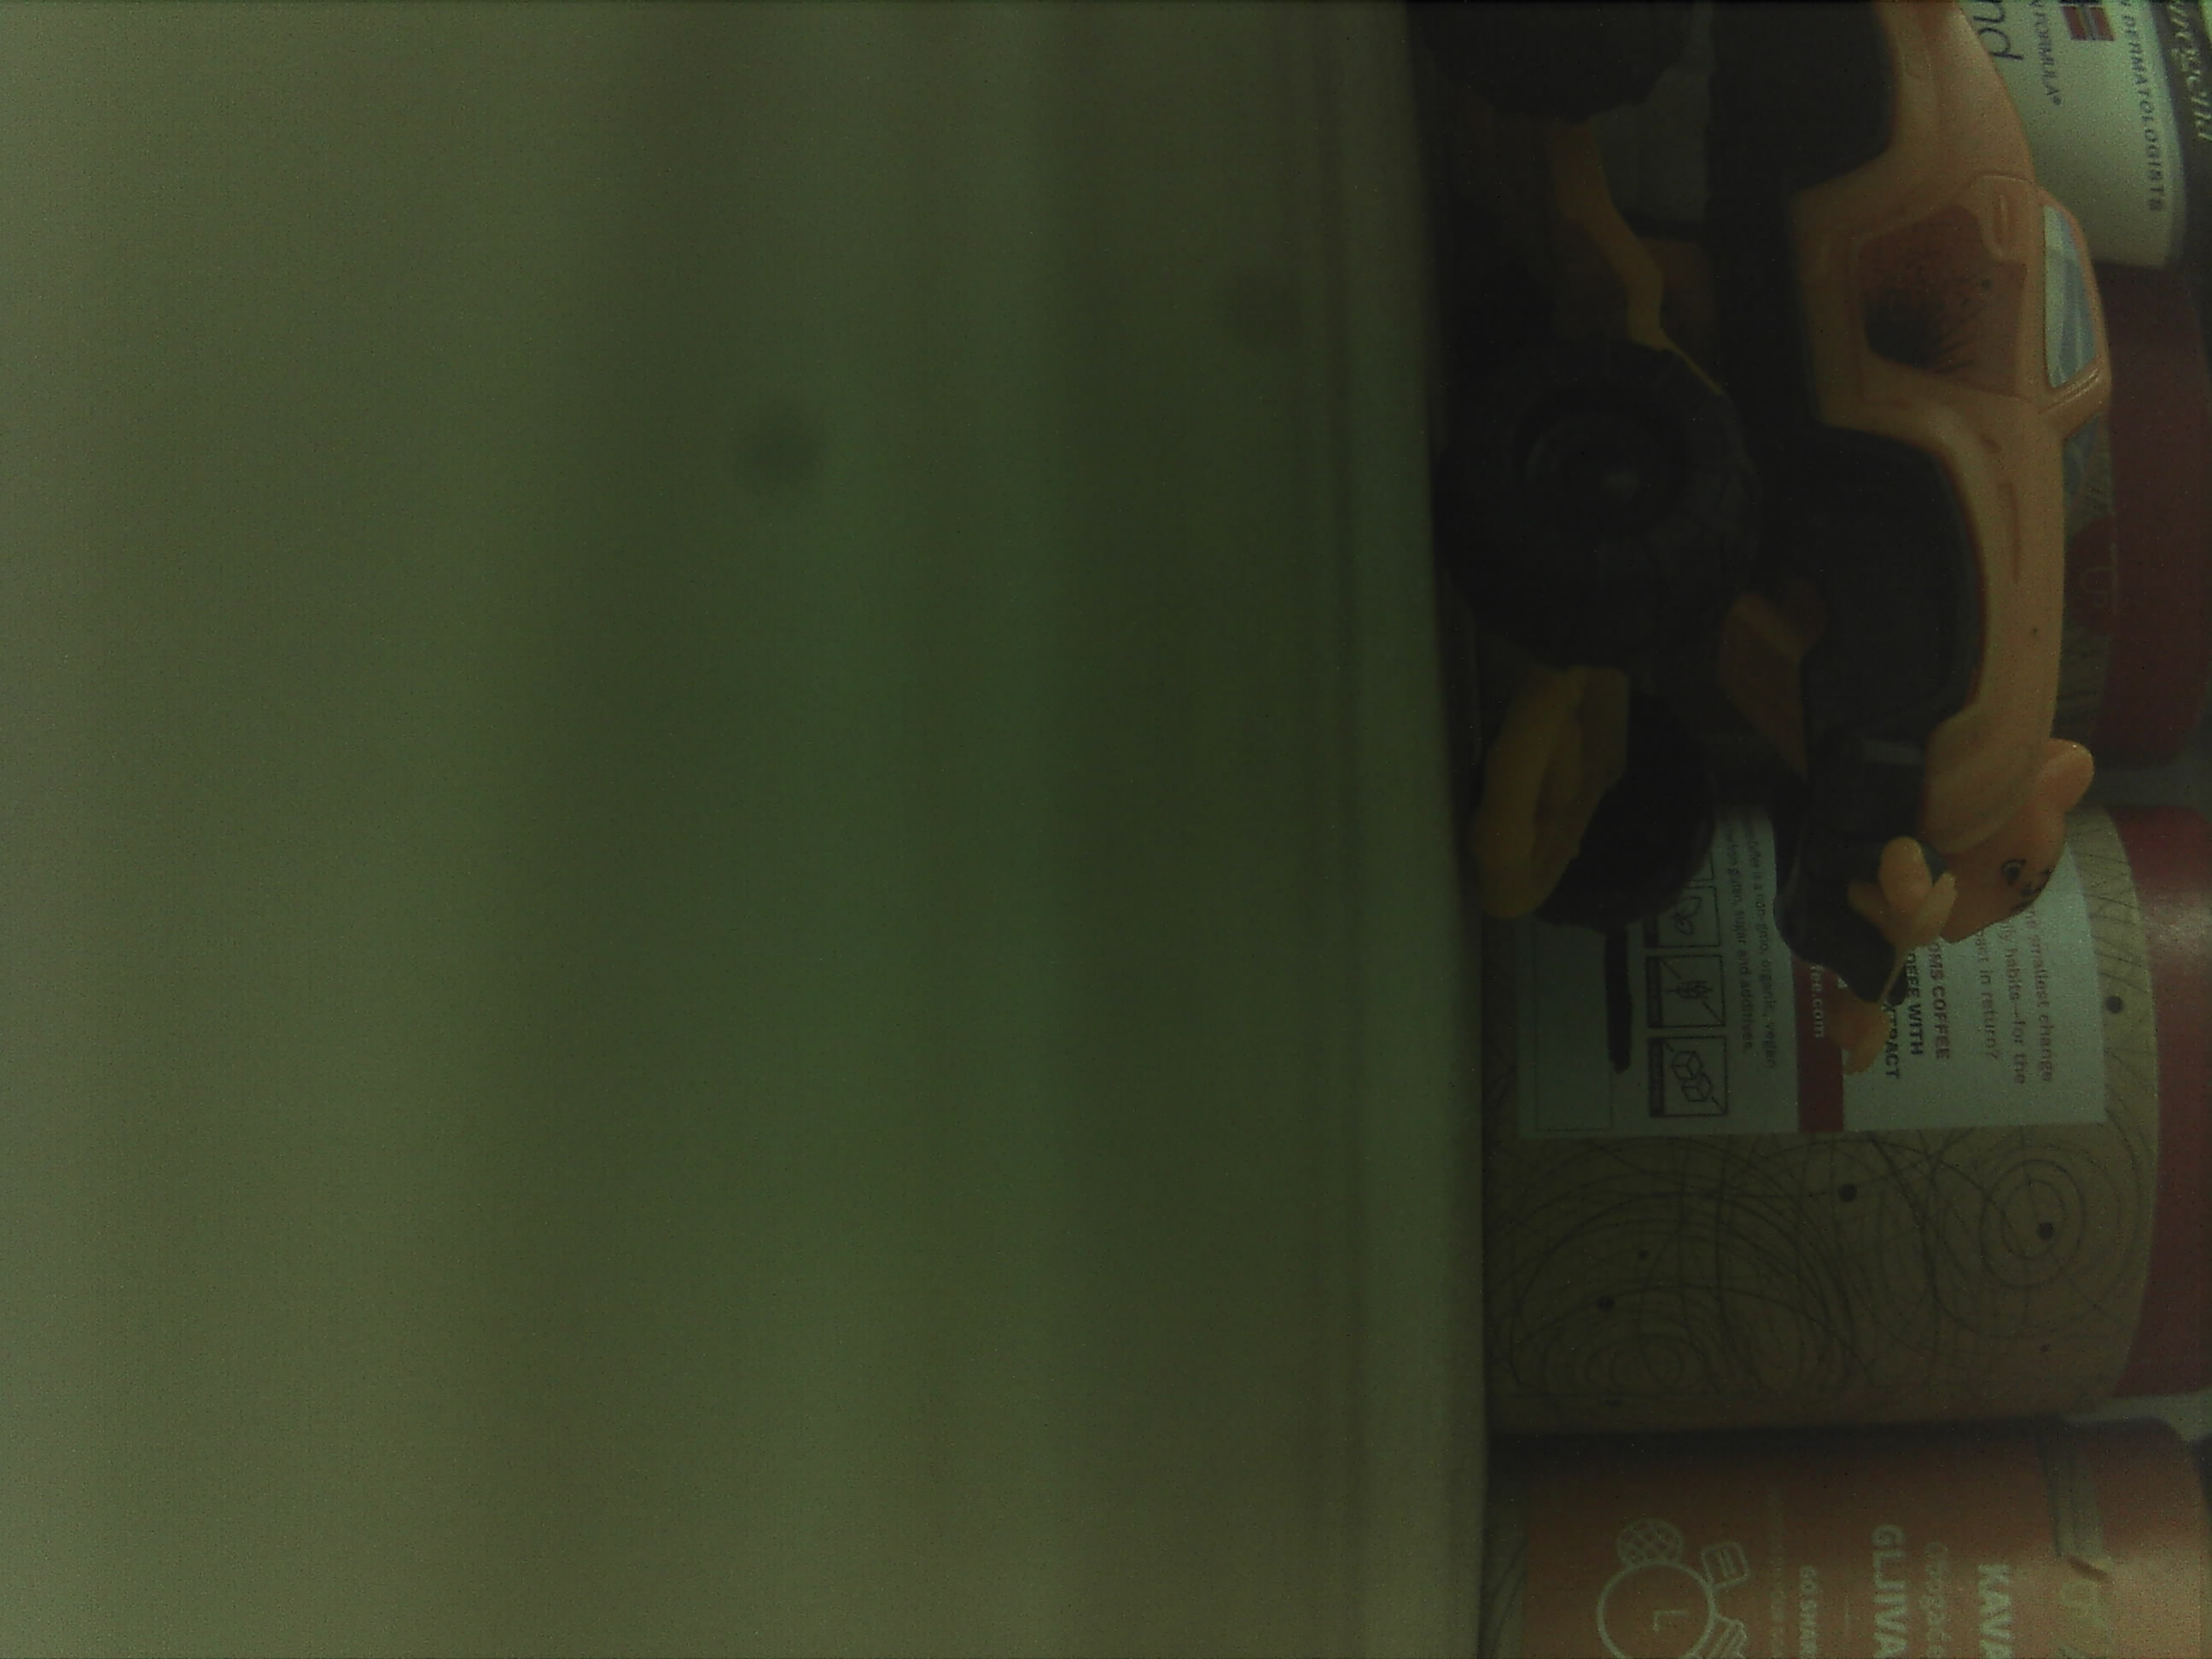
\includegraphics[height=5 cm, angle=90]{dark.jpeg}
	\caption{Slika dobivena u relativno mračnim uvjetima}
	\label{fig:dark}
\end{figure}